\documentclass[../main.tex]{subfiles}
\begin{document}
\setchapterstyle{kao}
\setchapterpreamble[u]{\margintoc}
\chapter[Representation Theory]{Representation Theory\footnotemark[0]}
\labch{RT}
%INIZIO LEZIONE 20/05 
Previously, we convinced ourselves that the fundamental principles of quantum theory are pushing us to investigate \textbf{unitary representations} of the group of transformations we are interested in. To be more precise, basic principles of quantum theory are suggesting us to study \textbf{projective unitary representations} of the group of physically relevant transformations. But we understood that in many cases we can reduce to \textbf{true} unitary representations, so homomorphisms of unitaries which are exact up to a phase: we have seen the famous theorem by Bargmann [\refthm{bargmann}] which tells us that if a Lie group is connected, simply-connected and semi-simple (which is a condition of simplicty of the Lie algebra, so in the neighbourhood of the identity) then every projective unitary representation can be readjusted, up to a change of a phase, to be a \textbf{true} unitary representation. E.g. in the case of SU(2), which is simply connected because topologically is a three-dimensional sphere and semi-simple by direct computation, we realized that we can reduce to study unitary representations. If we have a Lie group that is not simply-connected, the most prominent example is SO(3), then we cannot directly apply Bargmann's theorem but we know that for every not simply-connected Lie group there is its universal covering which "covers it", in the technical sense that there is a Lie group homomorphism which is surjective towards the group we are interested in and such that the universal covering is simply connected and the kernel of this map is a discrete, normal, central subgroup of the big one. Even if it is not true for SO(3) and for not simply-connected groups that every projective unitary representation can be readjusted to a be \textbf{true} unitary representation, we can always lift the problem to the universal covering. For the universal covering, every projective unitary representation is readjusted to a unitary representation so we study the unitary representation of the universal covering but at the very end we select those which pass to the group we started with. In particular those whose kernel contains the kernel of the covering. All this together suggests that we have to study unitary representation of groups and possibly classify them.
\section{Fundamental definitions}
\underline{\textbf{Settings:}} unless otherwise stated, $V$ will be a finite dimensional vector space over $\mathbb{K}=\{\mathbb{R},\mathbb{C}\}$. We will consider GL$(V)\cong\textrm{GL}(n,\mathbb{K})$ and similarly its Lie algebra will be $\mathfrak{gl}(V)\cong\textrm{End}(V)\cong\textrm{Mat}(n,\mathbb{K})$.
\begin{definition}[Representation]\index{Representation}
\labdef{rep}
Let G be a (matrix) Lie group. A \textbf{finite dimensional (linear) representation} of G on $V$ is a \textbf{Lie group homomorphism}:
\[
\Pi:G\xrightarrow[]{{\color{black}\text{Lie hom}}}\text{GL}(V)
\]
Namely:
\begin{enumerate}
    \item $\Pi(gh)=\Pi(g)\Pi(h) \quad \forall g,h\in G$
    \item $\Pi$ is $C^{\infty}$-smooth
\end{enumerate}
\end{definition}
A natural question would be: why don't we focus immediately on unitary representations? The basic principles of quantum theory told us that we have to study unitary representations of groups, while here we are not requiring it for the moment. The reason is that there are some relevant groups, e.g the Poincaré group, which do not admit finite dimensional unitary representations; so we have to study the finite dimensional linear representations, which are not unitary, and then synthesize an infinite dimensional unitary representation. A mathematician would give another motivation: if we can do it in general at the same cost, do it in general.

Similarly we have a representation for the Lie algebra.
\begin{definition}
Let $\mathfrak{g}$ be a Lie algebra. A \textbf{finite dimensional (linear) representation} of $\mathfrak{g}$ on $V$ is a \textbf{Lie algebra homomorphism}:
\[
\pi:\mathfrak{g}\xrightarrow[]{{\color{black}\text{Lie hom}}}\mathfrak{gl}(V)
\]
Namely:
\begin{enumerate}
    \item $\pi$ is linear
    \item $\pi([X,Y])=[\pi(X),\pi(Y)] \quad \forall X,Y\in\mathfrak{g}$
\end{enumerate}
\end{definition}
From this viewpoint, representations are just a special case of homomorphisms (respectively Lie group and Lie algebra homomorphisms) but in a special group, the general linear group of a vector space or its Lie algebra. 

When is a representation faithful\marginnote{Faithful is just a synonymous of injective.}?
\begin{definition}[Faithful]\index{Faithful}
A representation $\Pi$ (resp. $\pi$) is called \textbf{faithful} if it is \textbf{injective}:\marginnote{The arrow $\rightarrowtail$ means "injective"

The arrow means $\rightarrowtail>$ "injective and surjective"}
\[
G\overset{\Pi}{\rightarrowtail>}\Pi\underset{\mathclap{\tikz \node {$\uparrow$} node [below=1ex] {\footnotesize faithful copy of G };}}(G)\subseteq\text{GL}(V)
\]
\end{definition}
In this way, we do not lose information when looking at $\Pi(G)$ instead of G.

Now we have to define when is a representation irreducible and it is similar to what we have already seen for a Lie algebra or a Lie group in \vrefdef{Irreducible-Lie-algebra}.
\begin{definition}[Irreducible representation =: irreps]\index{Irreducible representation:=irreps}
\marginnote{From now on, we will use "irreps" because "irreducible representation" is too long.}Let $\Pi$ be a linear representation:
\[
\Pi:G\xrightarrow[]{}\text{GL}(V)
\]
A subspace $W\le V$ is called \textbf{invariant} if 
\[
\Pi(g)w\in W \qquad \forall\;w\in W,\ \ \forall\;g\in G \qquad \Big|\Big|\quad \text{\parbox{1.3cm}{Invariant\\subspace}}
\]
and it is called \textbf{non-trivial} if $W\ne\{0\}$ and $W\ne V$. A representation is called \textbf{irreducible} if it does \underline{not} admit any non trivial invariant subspaces.
\end{definition}
The same definition applies for a Lie algebra representation $\pi:\mathfrak{g}\xrightarrow[]{}$End$(V)$.

Now we have to declare when we consider two representation equivalent.\marginnote{\cite{Hall2015} uses the word "isomorphic" but we prefer to use the word "equivalent".}
\begin{marginfigure}[10mm]
	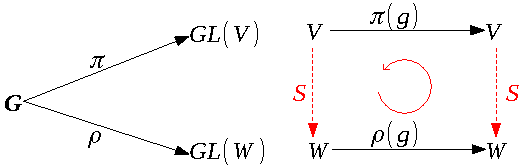
\includegraphics[width=1.2\linewidth]{images/intertwining.pdf}
	\caption[Interwining scheme]{"Intertwining" does not have a proper Italian translation. The colleagues from the previous generation use "intrallacciamento", the modern generation uses "mappa d'intreccio".}
	\labfig{intertwining}
\end{marginfigure}
\begin{definition}[Intertwining map]\index{Intertwining map}
An \textbf{intertwining map} between two representations $\pi$ and $\rho$ is a \textbf{linear operator} $S:V\xrightarrow[]{}W$ such that the diagram [\reffig{intertwining}] commutes, i.e. 
\[
\rho(g)S=S\pi(g) \quad \forall g\in G \qquad \Big|\Big|\quad \text{\parbox{1.3cm}{\centering Intertwining\\map}}
\]
If it is \underline{\textbf{invertible}} it is called an \textbf{isomorphism/equivalence of representations}. Notice that if \[
\rho(g)=S\pi(g)S^{-1} \quad \forall g\in G
\]
then we say that $\rho$ and $\pi$ are \textbf{isomorphic/equivalent.}
\end{definition}
If $S$ is unitary, which requires the fact that $V$ is an Hilbert space and this is not in our settings, we will say that they are \textbf{unitary equivalent} and this is what is really relevant to quantum theory. The idea is to classify representations of relevant groups up to unitary equivalence, so if two representations are unitary equivalent we will say that, for our purposes, they are the same representation. 

As we always said, in the theory of Lie groups the information flows very naturally from the group to the algebra. The vice-versa is difficult because locally there is a one-to-one correspondence, but not globally. The same happens for representations: a Lie group representation induces a Lie algebra representation, the vice-versa is subtler. With our approach this will be a corollary of what we have already understood for homomorphisms.
\begin{proposition}[Induced Lie algebra representations]\index{Induced Lie algebra representations}
Given a Lie group representation $\Pi:G\xrightarrow[]{}\text{GL}(V)$ there exists a \textbf{unique} Lie algebra representation $\pi:\mathfrak{g}\xrightarrow[]{}\mathfrak{gl}(V)$ such that:
\[
{\color{red}\Pi(e^x)=e^{\pi(x)} \quad \forall x\in\mathfrak{g} \quad || \quad \star}
\]
In particular:
\[
\pi(x)=\dv{}{t}\Pi(e^{tx})\Bigr|_{\substack{t=0}}=\dd\Pi\Bigr|_{\substack{e}}
\]
\end{proposition}
\begin{proof}
This is more a corollary than a proposition, notice that\\ $\Pi:G\xrightarrow[]{}\text{GL}(V)$ is a Lie group homomorphism and apply the corresponding result from \refthm{ind-homo}.
\end{proof}
\begin{kaobox}[frametitle=Remark]
\circled{1} Things are subtler in the other direction. In the sense that the Lie algebra representation fixes the Lie group representation in a neighbourhood of the identity but it is not clear in general so we should do a case-to-case study to understand if this local Lie group representation extends to a global one. As we move far away from the identity things become more complicated. E.g. for SU(2) every Lie algebra representation extends to a Lie group representation but this is not true for SO(3).\\
\circled{2} Does any Lie algebra representation come from a Lie group representation? In general no, but it does if G is \textbf{simply-connected (and connected)}. Again, we find one of the conditions of Bargmann's theorem [\vrefthm{bargmann}]. In our definition, which is the same as \cite{Hall2015}, a manifold is simply-connected if it is connected and every continuous path is continuously contractible to zero.
\end{kaobox}
Although the information from the Lie algebra to the Lie group does not flow so smoothly as in the other direction, there are still two important things which relate the two representations.
\begin{proposition}Let\marginnote{They are not independent}
\begin{align*}
    \Pi&:G\xrightarrow[]{{\color{red}\text{Lie hom}}}\text{GL}(V)\\
    \pi&:\mathfrak{g}\xrightarrow[]{{\color{red}\text{Lie hom}}}\mathfrak{gl}(V)
\end{align*}
where $\pi=\dd\Pi\Bigr|_{\substack{e}}$. Then:
\[
\begin{split}
\underset{\text{is irrep}}{\Pi}&\Longleftrightarrow\underset{\text{is irrep}}{\pi}\\
\underset{\text{are equivalent}}{\Pi_1\;\text{ and }\;\Pi_2}&\Longleftrightarrow\underset{\text{are equivalent}}{\pi_1\text{ and }\pi_2}
\end{split}
\]
\end{proposition}
\begin{definition}[Unitary representation]\index{Unitary representation}
Let $(V,\langle\dots,\dots\rangle):=\mathcal{H}$. A representation $\Pi:G\xrightarrow[]{}\text{GL}(V)$ is \textbf{unitary} if $\Pi(g)\in\pazocal{U}(\mathcal{H})$ for every $g\in G$, where $\pazocal{U}(\mathcal{H})$ is the group of unitary operators on $\mathcal{H}$.
\end{definition}
Does every group admit a finite dimensional unitary representation? As anticipated, the answer is no, we can recover unitarity with infinite dimensional representations.
%49:20
\section{Examples}
\subsection{Trivial representations}
This is the most trivial example, which always exists.
\[
\begin{cases}
\text{Group}: \Pi(g)=\mathbb{1}_V \quad &\forall g\in G\\
\text{Algebra}: \pi(x)=0 \quad &\forall x\in\mathfrak{g}
\end{cases}
\]
For the algebra it is zero since we have to take a derivative of something which is constant.
\subsection{Standard/defining representation of a matrix Lie group}
By definition, a matrix Lie group is a Lie group which, up to isomorphism, is a subgroup of the general linear group over the complex/real numbers $G\le\textrm{GL}(n,\mathbb{K})\simeq\textrm{GL}(\mathbb{K}^n)$. Matrix Lie groups have therefore a very natural representation. We define \[
\Pi_{\text{def}}:G\xrightarrow[]{}\text{GL}(\mathbb{K}^n)\quad  \text{with}\quad  \Pi_{\text{def}}(A)=A
\]
For example:
\begin{example}
\begin{align*}
    \text{SO}(3)&\xrightarrow[]{\Pi_{\text{def}}}\text{GL}(\mathbb{R}^3)\\
    \text{SU}(2)&\xrightarrow[]{\Pi_{\text{def}}}\text{GL}(\mathbb{C}^2)
\end{align*}
\end{example}
For every matrix Lie group there is always a defining representation.
\subsection{Adjoint operators}
Let G be a matrix Lie group and $\mathfrak{g}=\textrm{Lie}G\ni X$. The \textbf{adjoint action of $G$} is defined as:
\[
Ad_R(X):=RXR^{-1}\in\mathfrak{g} \quad
\]
This defines a representation, beacuse
\[
{\color{red}
\begin{split}
    Ad:&\;G\xrightarrow[]{}\text{GL}(\mathfrak{g})\\
    &\;R\mapsto Ad_R
\end{split}}
\]
\begin{exercise}
Check that $Ad_R\in\textrm{GL}(\mathfrak{g})$ by observing that\\ $(Ad_R)^{-1}=Ad_{R^{-1}}$ and $R\mapsto Ad_R$ is $\mathbb{C}^{\infty}$-smooth.
\end{exercise}
We have a nice representation of the group in the general linear group over its Lie algebra. Now we take the differential (infinitesimal symmetries) of it ${\color{red}ad:=\dd Ad\Bigr|_{\substack{e}}}$ and we obtain a representation of the Lie algebra in the endomorphism of the Lie algebra itself. This is remarkable: every Lie algebra can be represented over itself. 
{\color{red}
\begin{align*}
    ad:&\;\mathfrak{g}\xrightarrow[]{}\text{End}(\mathfrak{g})\\
    &\;x\mapsto ad_x
\end{align*}}
with the property ${\color{red}ad_X(Y)=[X,Y] \quad (\star)}$.

{\fontencoding{U}\fontfamily{futs}\selectfont\char 66\relax} Every (matrix) Lie group has a non trivial representation on its Lie algebra by \textbf{conjugation}. Every Lie algebra has a non trivial representation on itself by {\color{red}$ad_X(\cdot)=[X,\cdot]$}.

\underline{\textbf{Remark:}} We used this fact when when we defined $\Phi_U(X)=UXU^{-1}$ [\reflemma{phiuxu}] with $X\in V=i\mathfrak{su}(2)$ \textit{morally} $\mathfrak{su}(2)$.\marginnote{i$\mathfrak{su}(2)$ is the $\mathfrak{su}$(2) of physicists. [\refsec{importancei}]}
\section{Direct sums}
\begin{definition}
Given two representations:
\[
\begin{cases}
\Pi_1:G\xrightarrow[]{}\text{GL}(V_1)\\
\Pi_2:G\xrightarrow[]{}\text{GL}(V_2)
\end{cases}
\]
we define the \textbf{direct sum} {\color{black}$\Pi_1\oplus\Pi_2$}:
\[
\Pi_1\oplus\Pi_2:G\xrightarrow[]{}\text{GL}(V_1\oplus V_2)
\]
more formally:
\[
{\color{black}(\Pi_1\oplus\Pi_2)(R)}(V_1,V_2):=\left({\color{black}\Pi_1(R)}V_1,\;{\color{black}\Pi_2(R)}V_2\right) \quad \forall R\in G
\]
\end{definition}
\begin{kaobox}[frametitle=Remark]
In practice,
\[
(\Pi_1\oplus\Pi_2)(R)=\left(\begin{array}{c:c}
\Pi_1(R) & 0\\
\hdashline
0 & \Pi_2(R)
    \end{array}\right)
\]
By iteration, one defines $\bigoplus_{j=1}^N\Pi_j$ on $\bigoplus_{j=1}^NV_j$
\end{kaobox} 
\section[Reducibility and Schur's lemma]{Reducibility and \href{https://en.wikipedia.org/wiki/Issai_Schur}{Schur}'s lemma}
\begin{marginfigure}
	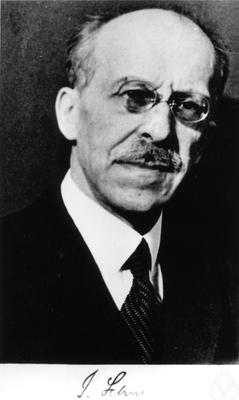
\includegraphics[width=1\linewidth]{images/Schur.jpg}
	\caption[Photo of Issai Schur]{From \href{https://en.wikipedia.org/wiki/Issai_Schur\#/media/File:Schur.jpg}{Wikimedia:} Issai Schur (10 January 1875 – 10 January 1941) was a Russian mathematician who worked in Germany for most of his life.}
	\labfig{schur}
\end{marginfigure}
\begin{definition}[Complete reducibility]\index{Complete reducibility}
A finite dimensional representation of a Lie (group or algebra) is called \textbf{completely reducible} if it is equivalent/isomorphic to a \textbf{direct sum of finitely many irreps}, i.e. $\exists\;S$ isomorphism such that:
\[
S\Pi(g)S^{-1}=\Big(\bigoplus_{j=1}^N\underset{\mathclap{\tikz \node {$\uparrow$} node [below=1ex] {\footnotesize \underline{\textbf{irreps!!}} };}} {\rho_{j}}\Big)(g)
\]
\end{definition}
This definition is a property of the pair (Lie group/algebra, representation). If this is true for every representation then it is a property of the Lie group/algebra.
\begin{definition}
A Lie (group or algebra) has the \textbf{complete reducibility property} if \underline{every} finite dimensional representation is completely reducible.
\end{definition}
{\fontencoding{U}\fontfamily{futs}\selectfont\char 66\relax} Not every Lie group has this property! 
\begin{example}
For example, $G=(\mathbb{R},+)$ is extremely easy but it is \textbf{not compact}. 

Consider $\Pi:\mathbb{R}\xrightarrow[]{{\color{red}\text{Lie hom}}}\text{GL}(\mathbb{C}^2)$:
\[
\Pi({\color{red}x})=\left(\begin{array}{cc}
    1 & {\color{red}x} \\
    0 & 1
    \end{array}\right)\quad
\xrightarrow[]{} \text{the span of $\varepsilon_1=\begin{pmatrix}1\\0\end{pmatrix}$ is invariant}
\]
If the representation were reducible, we should be able to find another one-dimensional subspace, which is invariant, and then prove that the representation is the direct sum of two subrepresentations: one is trivial and the other will contain all the information.
\end{example}
\begin{exercise}
Check that the only invariant subspaces are: $\{0\}$, $\text{span}(\varepsilon_1)$, $\mathbb{C}^2$.
\end{exercise}
It is clear that we cannot reduce by a dimensionality problem, because in order to have a reduction we would need two one-dimensional invariant subspaces, in such a way that the direct sum of the representation gives the original one and we do not have the second addendum, i.e. there is no other one-dimensional subspace which is invariant.

Even the easiest Lie group $\mathbb{R}$ is not completely reducible and the problem is the lack of compactness and we will see [\refthm{Weyl}] that things are much better for compact Lie groups.

Now we are going to see that all representations are equal but some representations are more equal than others.\marginnote{From George Orwell's \href{https://en.wikipedia.org/wiki/Animal_Farm}{Animal Farm}: \textit{all animals are equal but some animals are more equal than others}.}
\begin{proposition}[Unitary representation are completely reducible]\index{Unitary representation are completely reducible}
\labprop{unirep}
Let $\Pi:G\xrightarrow[]{{\color{red}\text{Lie hom}}}\pazocal{U}(\mathcal{H})$ with $\dim\mathcal{H}<\infty$. Then $\Pi$ is \textbf{completely reducible}. 

Similarly, if $\pi:\mathfrak{g}\xrightarrow[]{{\color{red}\text{Lie hom}}}\mathfrak{gl}(\mathcal{H})$ which is "unitary" (i.e. $\pi(x)^*=-\pi(x)$). Then $\pi$ is \textbf{completely reducible}.
\end{proposition}
Unitary representations are our friends because they are inspired by the basic principles of quantum theory and because they are simpler, they are completely reducible. What about the other groups? It turns out that every compact Lie group has the complete reducibility property and there is a beautiful theorem by \href{https://en.wikipedia.org/wiki/Hermann_Weyl}{Hermann Weyl} called \textit{unitarization trick}. He understood how to convert any linear representation of a compact Lie group into a unitary one and this is what we are going to see.
\begin{marginfigure}
	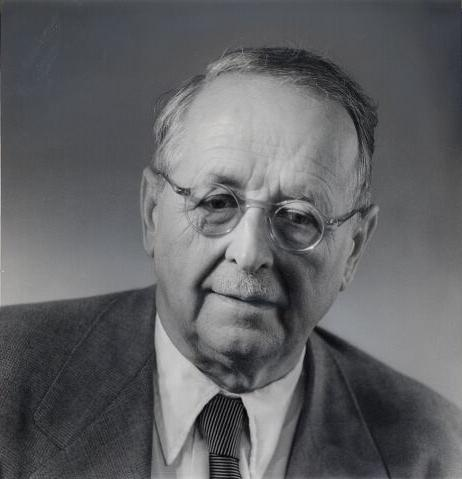
\includegraphics[width=1.2\linewidth]{images/Hermann_Weyl_ETH-Bib_Portr_00890.jpg}
	\caption[Photo of Hermann Klaus Hugo Weyl]{From \href{https://commons.wikimedia.org/wiki/File:Hermann_Weyl_ETH-Bib_Portr_00890.jpg}{Wikimedia:} Hermann Klaus Hugo Weyl, (9 November 1885 – 8 December 1955) was a German mathematician, theoretical physicist and philosopher.}
	\labfig{weyl}
\end{marginfigure}
\begin{theorem}[Weyl]\index{Weyl}
\labthm{Weyl}
If G is a \underline{\textbf{compact}} (matrix) Lie group, then every finite dimensional representation is \textbf{completely reducible}.
\end{theorem}
\raisebox{-\mydepth}{{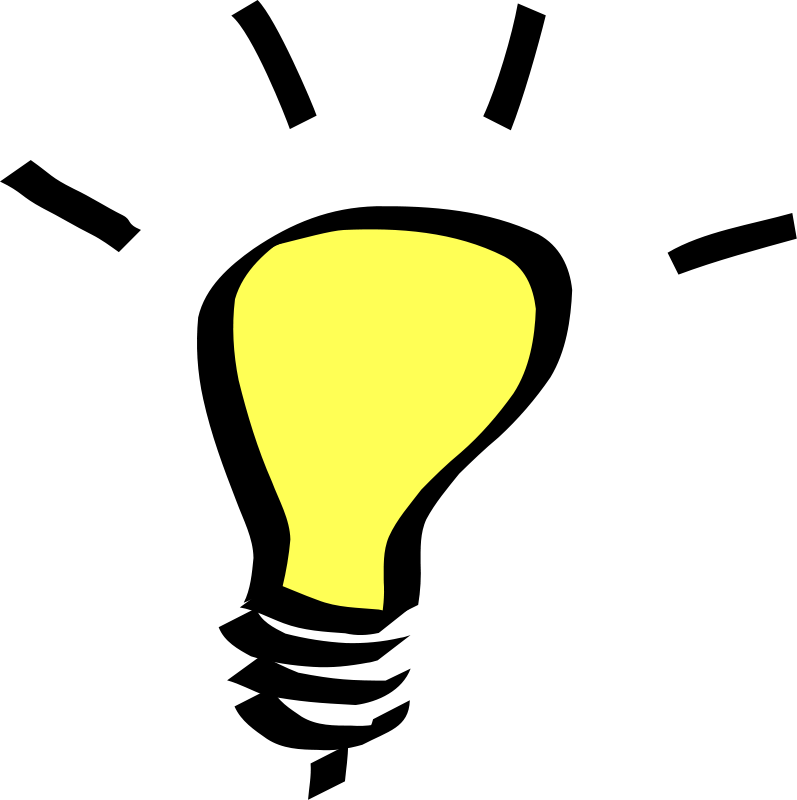
\includegraphics[height=1.1\baselineskip]{images/lamp.png}}} \underline{\textbf{Idea:}} Weyl's unitarization trick.
\begin{proof}
Consider finite representation $\Pi:G\xrightarrow[]{{\color{red}\text{Lie hom}}}\text{GL}(V)$, in general this is not a unitary representation. The idea by Weyl was to define an inner product, which depends on $G$ in such a way that it becomes a unitary representation with respect to this inner product. Therefore, we construct an inner product (sesquilinear, hermitian, positive definite) $\langle\dots,\dots\rangle_{\color{red}G}$ \textbf{depending on} $G$ (and also on $\Pi$) such that:
\[
\langle\Pi(g)v,\;\Pi(g)w\rangle_{\color{red}G}=\langle v,w \rangle_{\color{red}G} \quad \forall g\in G
\]
Once we proved that the representation with respect to this special inner product is unitary, we can apply \refprop{unirep} and we are done.

This inner product will be a sort of average of the inner product over the group and in order to construct this average we have to integrate over the group, therefore we need a volume form on G. Tentatively, we want:
\begin{equation}
\labeq{innerproduct}
{\color{red}\underset{\textrm{idea}}{\star}\quad \Big|\Big|}\qquad\langle v,w \rangle_{\color{red}G}:=\int_{\color{red}G}\overbrace{\langle {\color{red}\Pi(R)}v,{\color{red}\Pi(R)}w\rangle}^{\text{any inner product}}\dd\mu\underset{\mathclap{\tikz \node {$\uparrow$} node [below=1ex] {\footnotesize \parbox{3.5cm}{We need a \textbf{volume form on G invariant under translations}}};}}({\color{red}R})
\end{equation}
%1:39:52
\circled{1} Volume form on $G$:\marginnote{Here the theory of differential forms appears (\refch{diff_form_I} and \refch{diff_form_II})}

How do we define it? A volume form is a differential form of maximal degree, let's say $\dim G=k$. We then want to define a $k$-form which is the assignment at every point of an alternating $k$-linear form on every tangent space. One prominent tangent space is the tangent space at the identity $\mathfrak{g}=T_{\mathbb{1}}G$ and then there will be all the other guys. It turns out that if we look at the tangent space at the point $R$ this will be related to the tangent space at the identity by this relation:
\[
Y\in T_RG=\{XR:X\in\mathfrak{g}\}\quad \xrightarrow[]{}YR^{-1}\;\in\mathfrak{g}
\]
$R$ is the fixed point, so we look at the tangent space to the group at the point $R$, we can repeat for any collection of vectors what we did for $Y_1$ and $Y_2$ in the picture below.
\begin{figure}[h!]
    \centering
    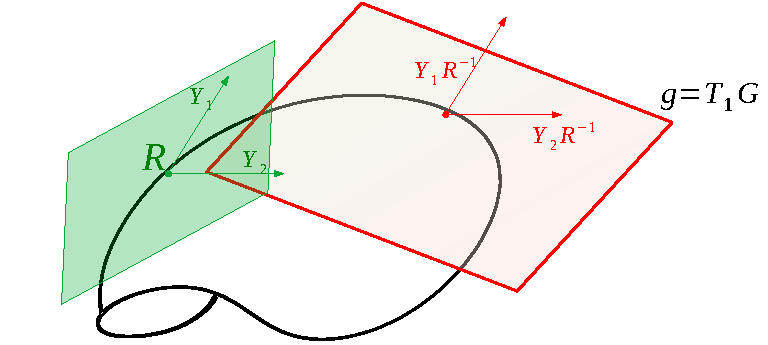
\includegraphics{images/tangentweyl.pdf}
    \caption*{}
    \labfig{tangentweyl}
\end{figure}
\marginnote{Some of you has found in the books another definition of the Lie algebra, stating that it is a set of all the left invariant vector fields. This definition comes from this observation: if we have the Lie algebra, we can define in this way vector fields over all the group which are left invariant by construction. The people from the books reversed the viewpoint and obtained this definition.}

We now choose an alternating k-linear form on $\mathfrak{g}$:
\begin{align*}
    \alpha_*:\mathfrak{g}\times\dots\times\mathfrak{g}&\xrightarrow[]{}\mathbb{R}\\
    (x_1,\dots,x_k)&\mapsto\alpha(x_1,\dots,x_k)\marginnote{This is the $\alpha$-volume of the parallelogram bounded by $x_1,\dots,x_k$.}
\end{align*}
Then we define a \textbf{differential k-form} $\alpha$\marginnote{Check that $\alpha$ is a differential k-form. It is possible to use a local basis in which $e_j\Bigr|_{\substack{R}}
=E_jR$, with $\{E_1,\dots,E_k\}$ a basis for the Lie algebra.}:
{\color{red}
\begin{align*}
    \alpha_R:T_RG\times\dots\times T_RG&\xrightarrow[]{}\mathbb{R}
\end{align*}
}
So this guy will be
\[
    {\color{red}\alpha_R(Y_1,\dots,Y_k)=}\underset{\mathclap{\tikz \node {$\uparrow$} node [below=1ex] {\footnotesize  acts on $\mathfrak{g}$};}}{{\color{red}\alpha_*}}{\color{red}(Y_1R^{-1},\dots,Y_kR^{-1}) \qquad \Big|\Big| \quad \star}
\]
\circled{2} Integrate on $G$:

Given $f:G\xrightarrow[]{{\color{red}C^0}}\mathbb{R}$ we can define \[
\int_{\color{red}G}f(R)\underbrace{\alpha(R)}_{\textrm{\parbox{1cm}{\centering Volume form}}}
\]
the function is a zero-form, the volume form is a $k$-form and it is possible to integrate over the group G which has dimension $k$. We observe by construction that it is \textbf{invariant under translations}:
\[
\int_{G}f(R{\color{red}S})\alpha(R)=\int_{G}f(R)\alpha(R)\quad \forall\;{\color{red}S}\in G \marginnote{Analogous to what we have for real valued functions:
\[
\int_{\mathbb{R}}f(x+a)\dd x=\int_{\mathbb{R}}f(x)\dd x\]
This holds true only because $\dd{x}$, which is a 1-form, is \textbf{invariant under translations}. It is a remarkable property of the Lebesgue and the Riemann integral, if we integrate with respect to the Gaussian measure it will not be invariant under translations.}
\]
We did not check that $\alpha(R)$ is invariant under translation but it is easy to see that from the way we constructed the volume form.

\circled{3} \textit{Unitarize} the representation:

We have to check that in \refeq{innerproduct} (which is no more a tentative):
\begin{enumerate}
    \item $\langle\dots,\dots\rangle_{G}$ is an inner product (exercise);
    \item $\Pi$ is unitary w.r.t. $\langle\dots,\dots\rangle_{G}$
\end{enumerate}
For every $S\in G$ we compute:
\WithArrowsOptions{displaystyle}
    \[
    \begin{WithArrows}
\langle\Pi(S)v,\Pi(S)w\rangle_{\color{red}G}&=\int_{G}\langle\Pi(S)\Pi(R)v,\Pi(S)\Pi(R)w\rangle\alpha(R)=\marginnote{Here we use the fact that $\Pi$ is a \textbf{representation} (property 1 of \refdef{rep}) and that $\alpha(R)$ is invariant under translation.}\Arrow{$\Pi$ hom}\\
&=\int_{G}\underbrace{\langle\Pi(SR)v,\Pi(SR)w\rangle}_{f(SR)}\alpha(R)=\\
&=\int_{G}f(R)\alpha(R)=\\
&=\langle v|w \rangle_{\color{red}G}
\end{WithArrows}
\]
Then $\Pi(S)$ is an \textbf{isometry}, hence \textbf{injective} and (for $\dim\mathcal{H}<\infty$) \textbf{surjective} $\Rightarrow\Pi(S)$ is \underline{\textbf{unitary}}. Once we proved it is unitary we can use \refprop{unirep} and we are done. 
\end{proof}
%FINE LEZIONE 20/05
%INIZIO LEZIONE 23 del 26/05/2022
Question: Where did we use the fact that the group $G$ \textbf{is compact}??

This hypothesis is crucial, because we exhibit a counterexample for the group of real numbers, which is non-compact. When checking that $\braket{\dots}_{G}$ is an inner product, in fact we have to check that $\braket{v}{w}_{G}{\color{red}\in\mathbb{C}}$ which follows by proving $\braket{v}_{G}=\norm{v}^2_{G}\,{\color{red}<+\infty}$. So, in a sense, we have to prove that the following guy is finite\marginnote{The volume form is non-negative by construction}
\WithArrowsOptions{displaystyle}
\[
    \begin{WithArrows}
    \norm{v}_{G}^2&=\int_{G}\overbrace{\braket{\Pi(R)v}}^{\ge 0}\alpha(R)=\\
    &=\int_{G}\underbrace{\norm{\Pi(R)v}^2}_{\ge 0}\underbrace{\alpha(R)}_{\text{\parbox{1cm}{\centering Volume form}}}\;{\color{red}\overset{?}{<}+\infty}
    \end{WithArrows}
\]
So we have a very simple inequality, and we estimate that guy from above
\[
\norm{v}_{G}^2\leq\underbrace{\sup_{{\color{red}R}\in G}\norm{\Pi({\color{red}R})}^2}_{\text{\centering\parbox{2cm}{$R\mapsto\norm{\Pi(R)}^2$ is \textbf{continuous}}}}\norm{v}^2\underbrace{\int_{{\color{red}G}}\alpha(R)}_{\text{\centering \parbox{1.5cm}{$\alpha$ is a \textbf{volume form}}}} 
\]
Now we use compactness twice: 
\begin{enumerate}
    \item First, to prove that the supremum is finte. Why? Because this is a continuous function over a compact set\marginnote{$\Pi$ is a Lie group representation, so it is a smooth function, the norm is always smooth and in particular continuous, therefore the map $R\to\norm{\Pi(R)}^2$ is continuous.}, hence by Weierstrass theorem is \textbf{bounded on a compact set} $G$.
    \item We are also using compactness for the second factor. It can be proved that our volume form is finite over the compact set, so it is a good measure.
\end{enumerate}
Hence\marginnote{The devil is in the details}
    \[
    \norm{v}_{G}^2\leq \max_{R\in G}\norm{\Pi(R)}^2\norm{v}^2\textrm{Vol}(G)<+\infty
    \]
\subsection{Schur's lemma (allotropic versions)}
The Schur's lemma is a fundamental tool is representation theory; there exist many versions of it. We present three versions: two as a theorem and one as a corollary.
\begin{theorem}[Schur]\index{Schur's lemma}\labthm{schur-lemma-v1}
Let $\Pi:G\to\textrm{GL}(V)$ be a \textbf{complex irreducible representation}. Suppose $\phi:V\to V$ is a linear operator that \textbf{commutes with the representation}, i.e.
\begin{equation}\labeq{schur-lemma-v1}
\star \quad \Big|\Big|\qquad \phi\Pi(g)=\Pi(g)\phi \quad \forall\;g\in G
\end{equation}
Then $\phi$ \textbf{is a multiple of the identity}, i.e. $\exists\;\lambda\in\mathbb{C}$ such that $\phi=\lambda\mathbb{1}$.
\end{theorem}
\begin{proof}
By contradiction: we negate the fact that $\phi$ is a multiple of the identity and we construct an invariant subspace. [We skip it for the lack of time]
\end{proof}
This is one possible version of the Schur's lemma, but we can also generalize it. We can think that the fundamental relation [\refeq{schur-lemma-v1}] can be read as the fact that $\phi$ intertwines the representation twice with itself. Now we could say "but we generalize it", we take two representation on the stage and to have an application $\phi$ which intertwines one with the other.\marginnote{An intertwining  is a linear map such that the diagram in \reffig{intertwining} is commutative}

Looking at \reffig{intertwining} we can generalize it a little bit more, distinguishing between $\phi_1$ and $\phi_2$. This more general version of Schur's lemma tells us that if $\phi_1$ and $\phi_2$ intertwine, then they are multiple of each other, up to a scalar. In particular we can take one of the two to be the identity, then if the two spaces are equal we will get back to version 1.
\begin{theorem}[Schur general]\index{Schur's lemma}\marginnote{We could spell it out algebraically, but we think it is easier to remember with the maps in \reffig{intertwining}}
Let $\phi_1$ and $\phi_2$ be \textbf{intertwining maps} between $\Pi:V\to V$ and $\rho:W\to W$. Then they are equal up to a scalar, i.e. $\exists\;\lambda\in\mathbb{C}$ such that
\[
\phi_2=\lambda\phi_1
\]
\underline{Special case}: $\Pi\equiv \rho$, $V=W$, $\phi_1=\mathbb{1}$ and $\phi_2=\phi$, we recover \refthm{schur-lemma-v1}.
\end{theorem}
Now we have a corollary, which it is also called \textit{Schur's lemma}.
\begin{corollary}[Schur's lemma]\index{Schur's lemma}\labcorol{schur-lemma}
Suppose $\Pi:G\to\textrm{GL}(V)$ is a \textbf{complex irreducible representation}. If we take an element $A\in Z(G)$\marginnote{Recall that the \textit{zentrum} $Z(G)=\left\{h\in G:\;hg=gh\quad \forall\;g\in G\right\}$. If a group is commutative, the \textit{zentrum} is all the group.} then the representation of this guy via $\Pi$ is a multiple of the identity, $\Pi(A)=\lambda\mathbb{1}$, \textbf{for some number} $\lambda\in\mathbb{C}$.
\end{corollary}
\begin{proof}
From \refthm{schur-lemma-v1}, observe that 
\[
\Pi(A)\Pi(g)=\Pi(Ag)\underset{\mathclap{\tikz \node {$\uparrow$} node [below=1ex] {\footnotesize $A\in Z(G)$};}}{=}\Pi(gA)=\Pi(g)\Pi(A)
\]
Choose $\phi=\Pi(A)\in\textrm{End}(V)$, from \refthm{schur-lemma-v1} we get that $\phi$ must be a multiple of the identity, i.e. ${\color{red}\exists\;\lambda\in\mathbb{C}:\quad \Pi(A)=\lambda\mathbb{1}}$
\end{proof}
Another important corollary for Quantum Mechanics is the following:
\begin{corollary}\marginnote{Actually there are not so many commutative Lie group, but the few ones are important. Ex: the group of space/momentum translations $G=\mathbb{R}^d$, or the d-dimensional torus $G=\Pi^d$, which is the group of quasi-momenta in solid state physics, or we could have direct product of that $G=\mathbb{R}^d\times\Pi^{d-k}$}
Suppose that $G$ is a \textbf{commutative Lie group}. Then every \textbf{irreducible representation is 1-dimensional}.
\end{corollary}
\begin{proof}
Suppose that $G$ is commutative. We fix $g\in G$. Then consider
\[
\Pi(g)\Pi(h)=\Pi(gh)\underset{\mathclap{\tikz \node {$\uparrow$} node [below=1ex] {\footnotesize $\Pi$ is commutative};}}{=}\Pi(hg)\overset{\mathclap{\tikz \node {$\downarrow$} node [above=1.25ex] {\footnotesize $\Pi$ is an homomorphism};}}{=}\Pi(h)\Pi(g)\qquad \forall\;h\in G
\]
So $\Pi(g)$ commutes with all the representations of the group. Then by the Schur's lemma in \refcorol{schur-lemma} (and therefore from \refthm{schur-lemma-v1}), $\phi=\Pi(g)$ is an intertwiner and it must be a multiple of the identity, i.e. $\exists\;\lambda_g=\lambda(g)$\marginnote{$\lambda(g)$ because it actually depends on $g$} such that
\[
{\color{red}\Pi(g)=\lambda(g)\mathbb{1} \qquad \forall\;g\in G}
\]
The element we focused on was generic, hence the representation\\
$g\mapsto\lambda(g)\in\mathbb{C}^\times$ is effectively a \textbf{1-dimensional irreducible representation}\marginnote{Every 1-dimensional representation is irreducible}.
\end{proof}
\begin{example}
Actually these one-dimensional representations are explicit in the example we mentioned in the note on the margin.
\begin{enumerate}
    \item 
    \begin{align*}
    \textrm{Irrep}(\mathbb{R}^d)
    &=\left\{\Pi:\mathbb{R}^d\xrightarrow[\textrm{Irred}]{\textrm{Lie hom}}\mathbb{C}^\times\right\}\marginnote{Since it must be an homomorphism, it must be continuous}\\
    &=\left\{\Pi_k: x\mapsto e^{ik\cdot x}\right\}_{k\in\hat{\mathbb{R}}^d}\\
    &=\textrm{ Plane waves, labelled by }k\in\hat{\mathbb{R}}^d
    \end{align*}
    Here is where all the Fourier theory starts.
    \item Similarly, if we study the irreducible representation of the d-dimensional torus\marginnote{This is like having a quantum particle on a circle: we will not have all the values of the momentum, but only thos who are compatible with the structure}
    \WithArrowsOptions{displaystyle}
    \[
    \begin{WithArrows}
    \textrm{Irreps}\left(\Pi^d\right)&\overset{\textrm{def}}{=}\left\{\Pi:\Pi^d_L\xrightarrow[\textrm{Irred}]{\textrm{Lie hom}}\mathbb{C}^\times\right\}\\
    &=\left\{\Pi_k:x\mapsto e^{ik\cdot x}\right\}_{k\in\frac{2\pi}{L}\mathbb{Z}^d}
    \end{WithArrows}
    \]
    Where $L$ is the length of the torus. We represent it in one dimension in \reffig{1dim_Tor}
    \[
    1=\psi(0)=\psi(2\pi)=e^{ikL}
    \]
\end{enumerate}
\end{example}
\begin{marginfigure}[-25mm]
	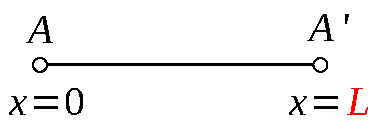
\includegraphics[width=1\linewidth]{images/1dim_Tor.pdf}
	\caption{One dimensional torus.}
	\labfig{1dim_Tor}
\end{marginfigure}
%44:00
\end{document}